

\documentclass[12pt, openright, twoside]{report}
% Language and encoding
\usepackage[utf8]{inputenc}
\usepackage[english]{babel}
% Page layout and margins
\usepackage[a4paper, margin=1in]{geometry}
% Graphics and captions
\usepackage{graphicx}                 % For including images
\usepackage{subcaption}               % For subfigures (if needed)
\usepackage[labelfont=bf, figurename=Fig., tablename=Table, font=small]{caption}
\captionsetup{font={small, stretch=1.2}} 

% Math and symbols
\usepackage{amsmath} % For advanced math commands
\usepackage{amssymb} % For additional symbols
\usepackage{bbold}   % For bold mathematical symbols
% References
\usepackage[backend=biber, sorting=none]{biblatex} % For references
\addbibresource{references.bib}                     % Point to your bibliography file
% Title and section formatting
\usepackage{titlesec}
\titleformat{\section}{\normalfont\Large\bfseries}{\thesection}{1em}{}
\titleformat{\subsection}{\normalfont\large\bfseries}{\thesubsection}{1em}{}
% Lists and tables
\usepackage{enumitem} % For custom lists
\usepackage{multirow} % For tables with merged rows
\usepackage{multicol} % For multi-column text (if needed)
% Typography improvements
\usepackage{microtype} % Improves text justification and spacing
% Custom margins for specific content
\usepackage{changepage} % To change margins for specific sections (e.g., images)
% Floating objects
\usepackage{float} % For precise positioning of floats
% Miscellaneous
\usepackage{comment} % To comment out large blocks of text
% TikZ and PGFPlots (if needed for graphs)
\usepackage{tikz} % For custom graphics
\usepackage{pgfplots} % For plots and charts
\pgfplotsset{compat=1.18}
% Reduce compilation time (useful for TikZ-heavy documents)
\usepgfplotslibrary{external}
\tikzexternalize
% Line spacing
\renewcommand{\baselinestretch}{1.5}
% Headers and footers (if customization is needed)
\usepackage{fancyhdr}
\pagestyle{fancy}
% Configure the fancy header
\renewcommand{\headrulewidth}{0.4pt} % Adds a horizontal line
\fancyhead[C]{Martina Arrighini, Luigi Babiski Arruda, Giorgio Cottini, Enrico Paciaroni}
\fancyfoot[C]{\thepage}
% Hyperlinks
\usepackage{hyperref}
\hypersetup{
    colorlinks=true,
    linkcolor=blue,
    filecolor=magenta,
    urlcolor=cyan,
    pdftitle={Group Project Report},
    pdfpagemode=FullScreen,
}

\begin{document}

%-------- Title page -------------------------------------------------------------------------------------------------------%

    \begin{titlepage}
        \centering
        
\includegraphics[width=0.3\textwidth]{images/logo_unipd.png}\par\vspace{1cm}
        {\scshape\LARGE Università degli Studi di Padova \par}
        \vspace{1.5cm}
        {\scshape\Large Master Degree Course in Computational Finance \par}
        \vspace{.2cm}
        {\scshape\large Regression and Time Series Models \par}
        \vspace{2cm}
        {\Large\bfseries Group Work 1 - Regression with CAPM Model\par}
        \vspace{2cm}
        Created by:\par
        {\itshape{Martina Arrighini, 2149799, martina.arrighini@studenti.unipd.it}\par}
        {\itshape Luigi Babiski Arruda, 2031997, luigi.babiskiarruda@studenti.unipd.it\par}
        {\itshape Giorgio Cottini, 2140740, giorgio.cottini@studenti.unipd.it \par}
        {\itshape Enrico Paciaroni, 2139678, enrico.paciaroni@studenti.unipd.it \par}
        \vfill
        Commissioned by:\par
        Prof.\ Massimiliano Caporin
        \vfill
        {\large A.Y. 2024/2025}
    \end{titlepage}

\setcounter{page}{1}

%-------- Assignment 1 -----------------------------------------------------------------------------------------------------%
\section*{Assignment 1}

%-------- Assignment 2 -----------------------------------------------------------------------------------------------------%
\section*{Assignment 2}
\begin{figure}[h]
    \centering
    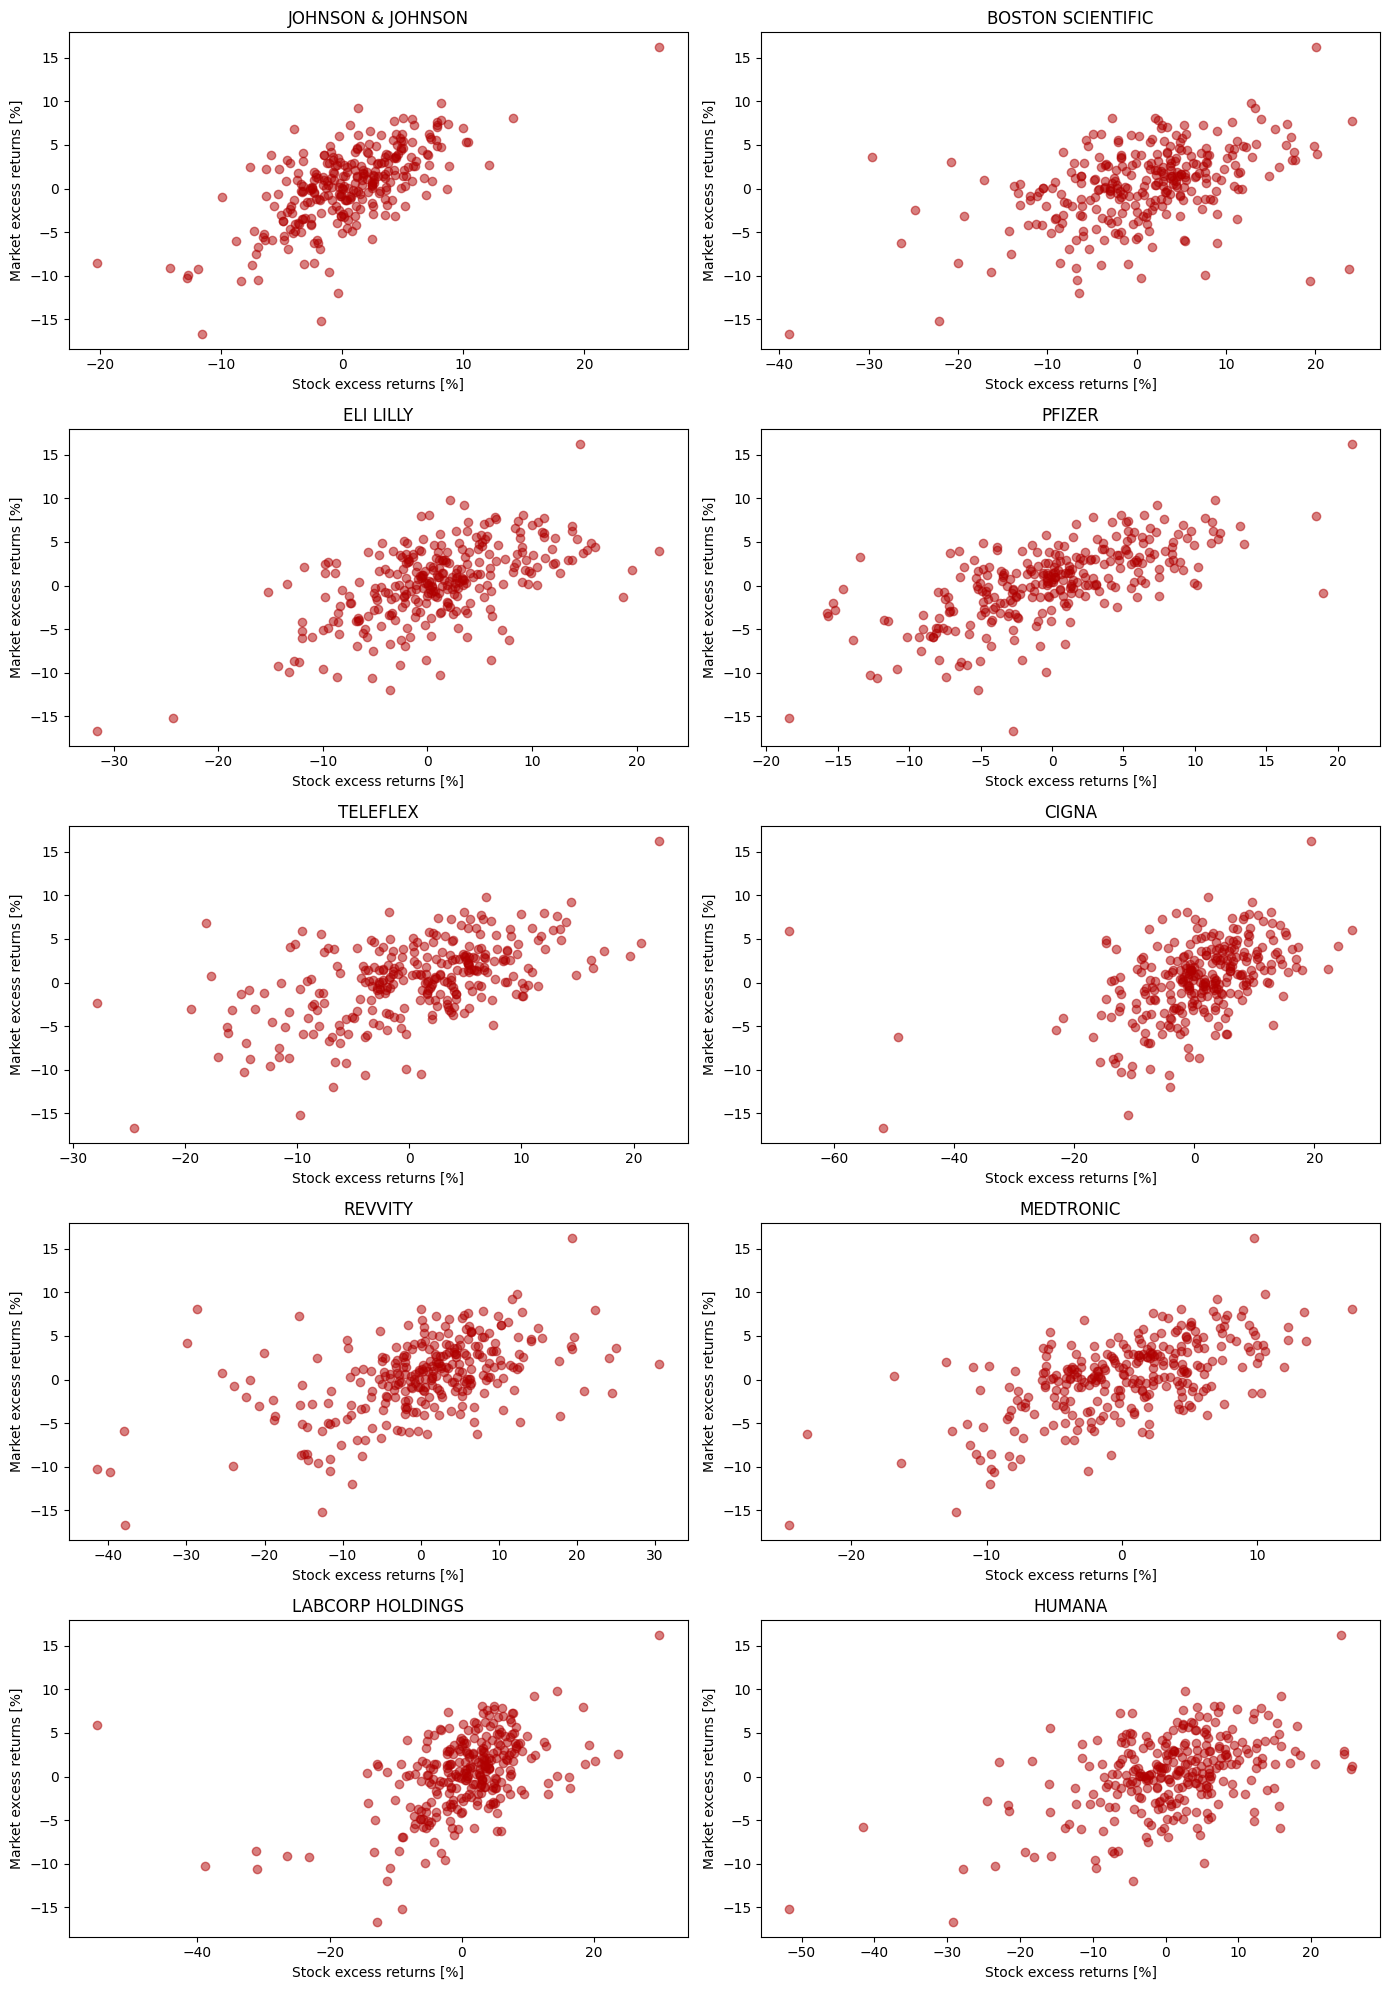
\includegraphics[width=0.8\textwidth]{images/equities_scatterplot.png}
    \caption{Scatterplot of equities' log-returns against excess market returns.}\label{fig:equities_scatterplot}
\end{figure}

%-------- Assignment 3 -----------------------------------------------------------------------------------------------------%
\section*{Assignment 3}
\begin{figure}[h]
    \centering
    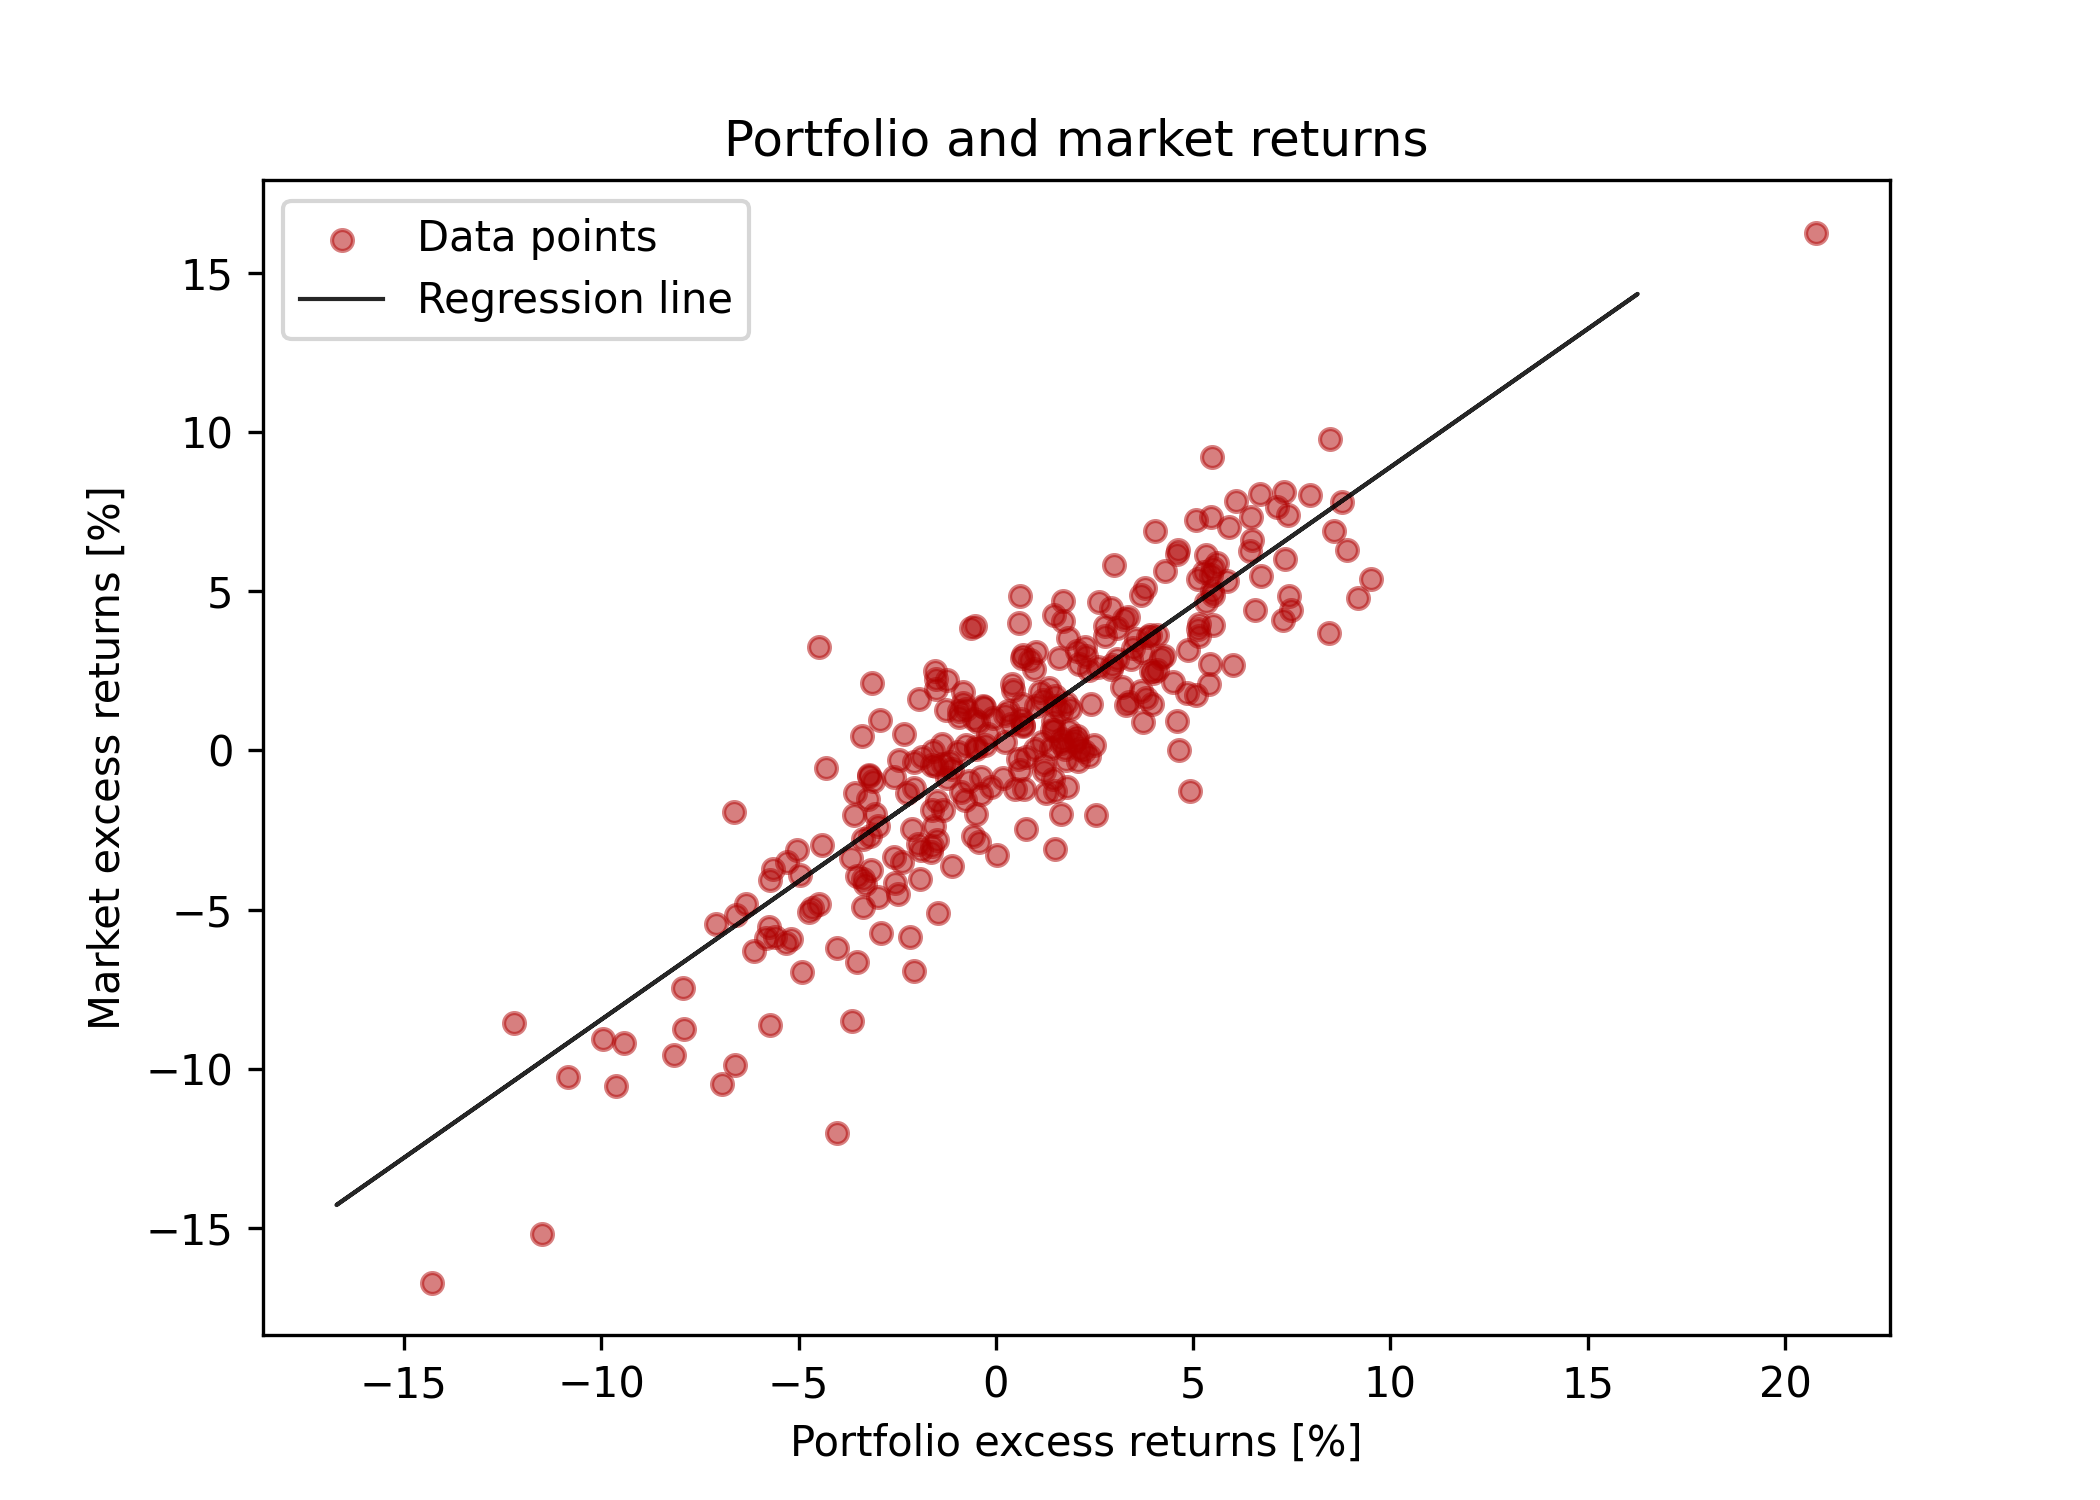
\includegraphics[width=0.8\textwidth]{images/portfolio_regression.png}
    \caption{Scatterplot of portfolio's returns against excess market returns, with linear regression.}\label{fig:portfolio_regression}
\end{figure}
%-------- Assignment 4 -----------------------------------------------------------------------------------------------------%
\section*{Assignment 4}

%-------- Assignment 5 -----------------------------------------------------------------------------------------------------%
\section*{Assignment 5}

In this section, we employ the Chow test to assess whether a significant structural change occurs in the regression models at 
specific points in time. 
To ensure the robustness of our analysis, we first established a minimum data subset size for the unrestricted models, 
setting it to 10\% of the total dataset, in order to maintain statistical validity while preserving sufficient data for
meaningful comparisons.
Subsequently, the Chow test was systematically applied to all linear regressions conducted on the selected equities, 
allowing us to identify potential structural breaks across the dataset, that is, significant changes in the regression
parameters caused by external shocks, market-wide events, or company-specific factors. 
These structural breaks may reflect shifts in the relationship between excess returns and market behaviour, such as changes in
systematic risk $(\beta)$ or the presence of unexplained excess returns $(\alpha)$ due to macroeconomic conditions, regulatory 
adjustments or sector-specific developments.
To identify these structural breaks, we analyzed the p-values obtained from the Chow test for each equity over time: 
a p-value below the threshold of 0.01 was interpreted as evidence of a structural break at that particular point in time,
signaling that the CAPM parameters had changed significantly.
The results of this analysis are presented in Figure~\ref{fig:chowmoving}.

\begin{figure}[h]
    \centering
    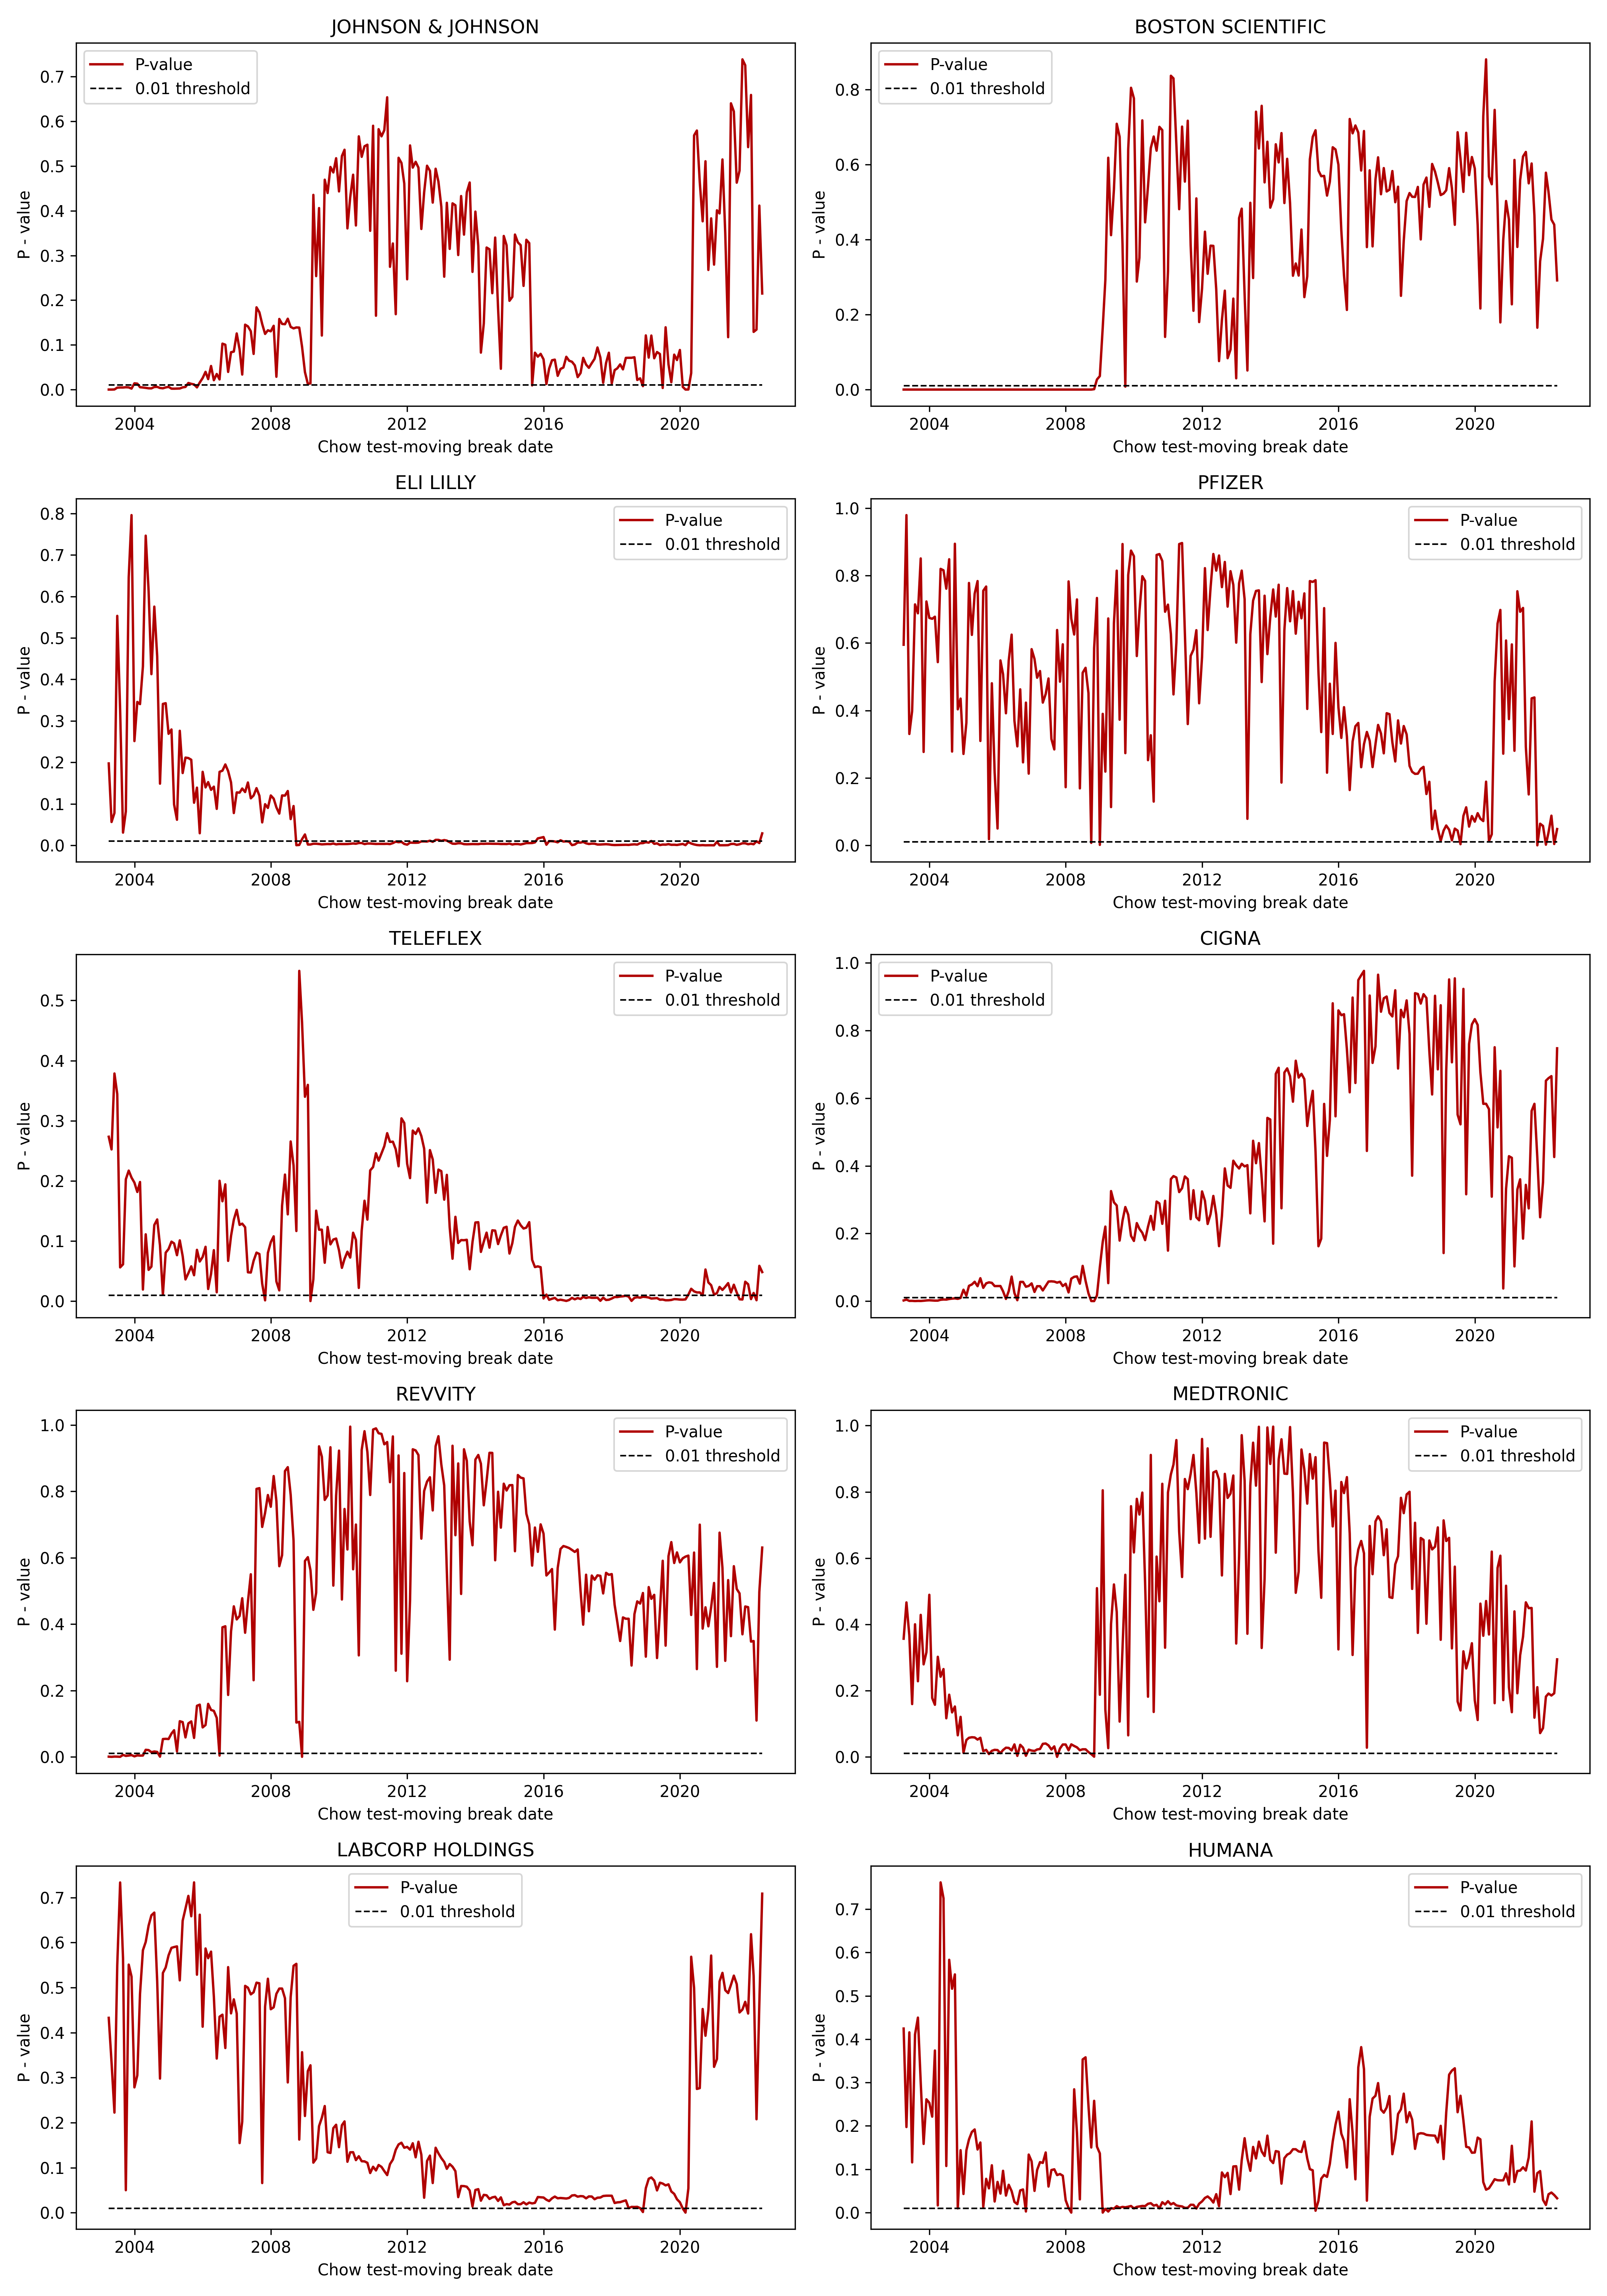
\includegraphics[width=0.8\textwidth]{images/chowmoving.png}
    \caption{Chow Test performed for all equities in search of structural breaks.}\label{fig:chowmoving}
\end{figure}

\begin{figure}[h]
    \centering
    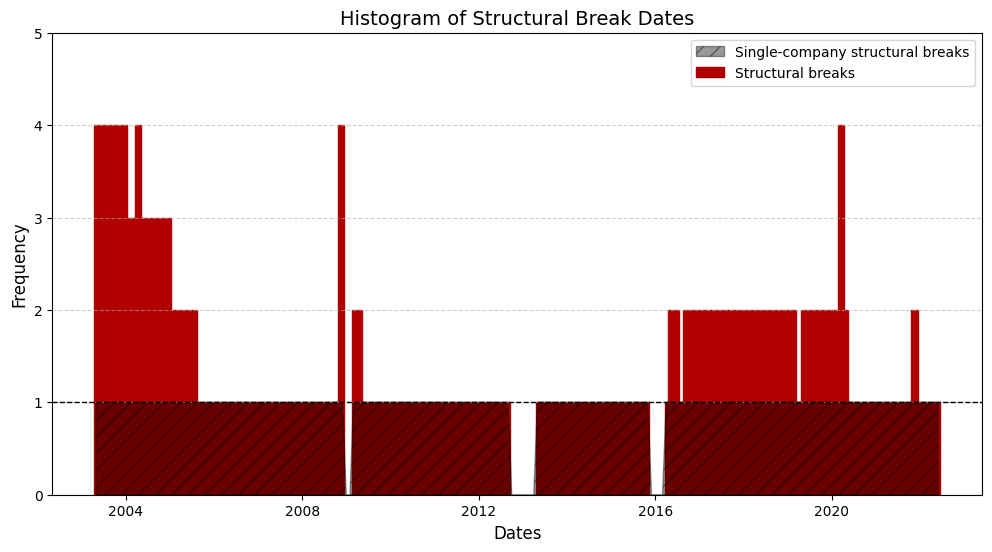
\includegraphics[width=0.8\textwidth]{images/struct_break_freqs.png}
    \caption{Frequency of months identified as structural break points.}\label{fig:struct_break_freqs}
\end{figure}
%-------- Assignment 6 -----------------------------------------------------------------------------------------------------%
\section*{Assignment 6}

\begin{figure}[h]
    \centering
    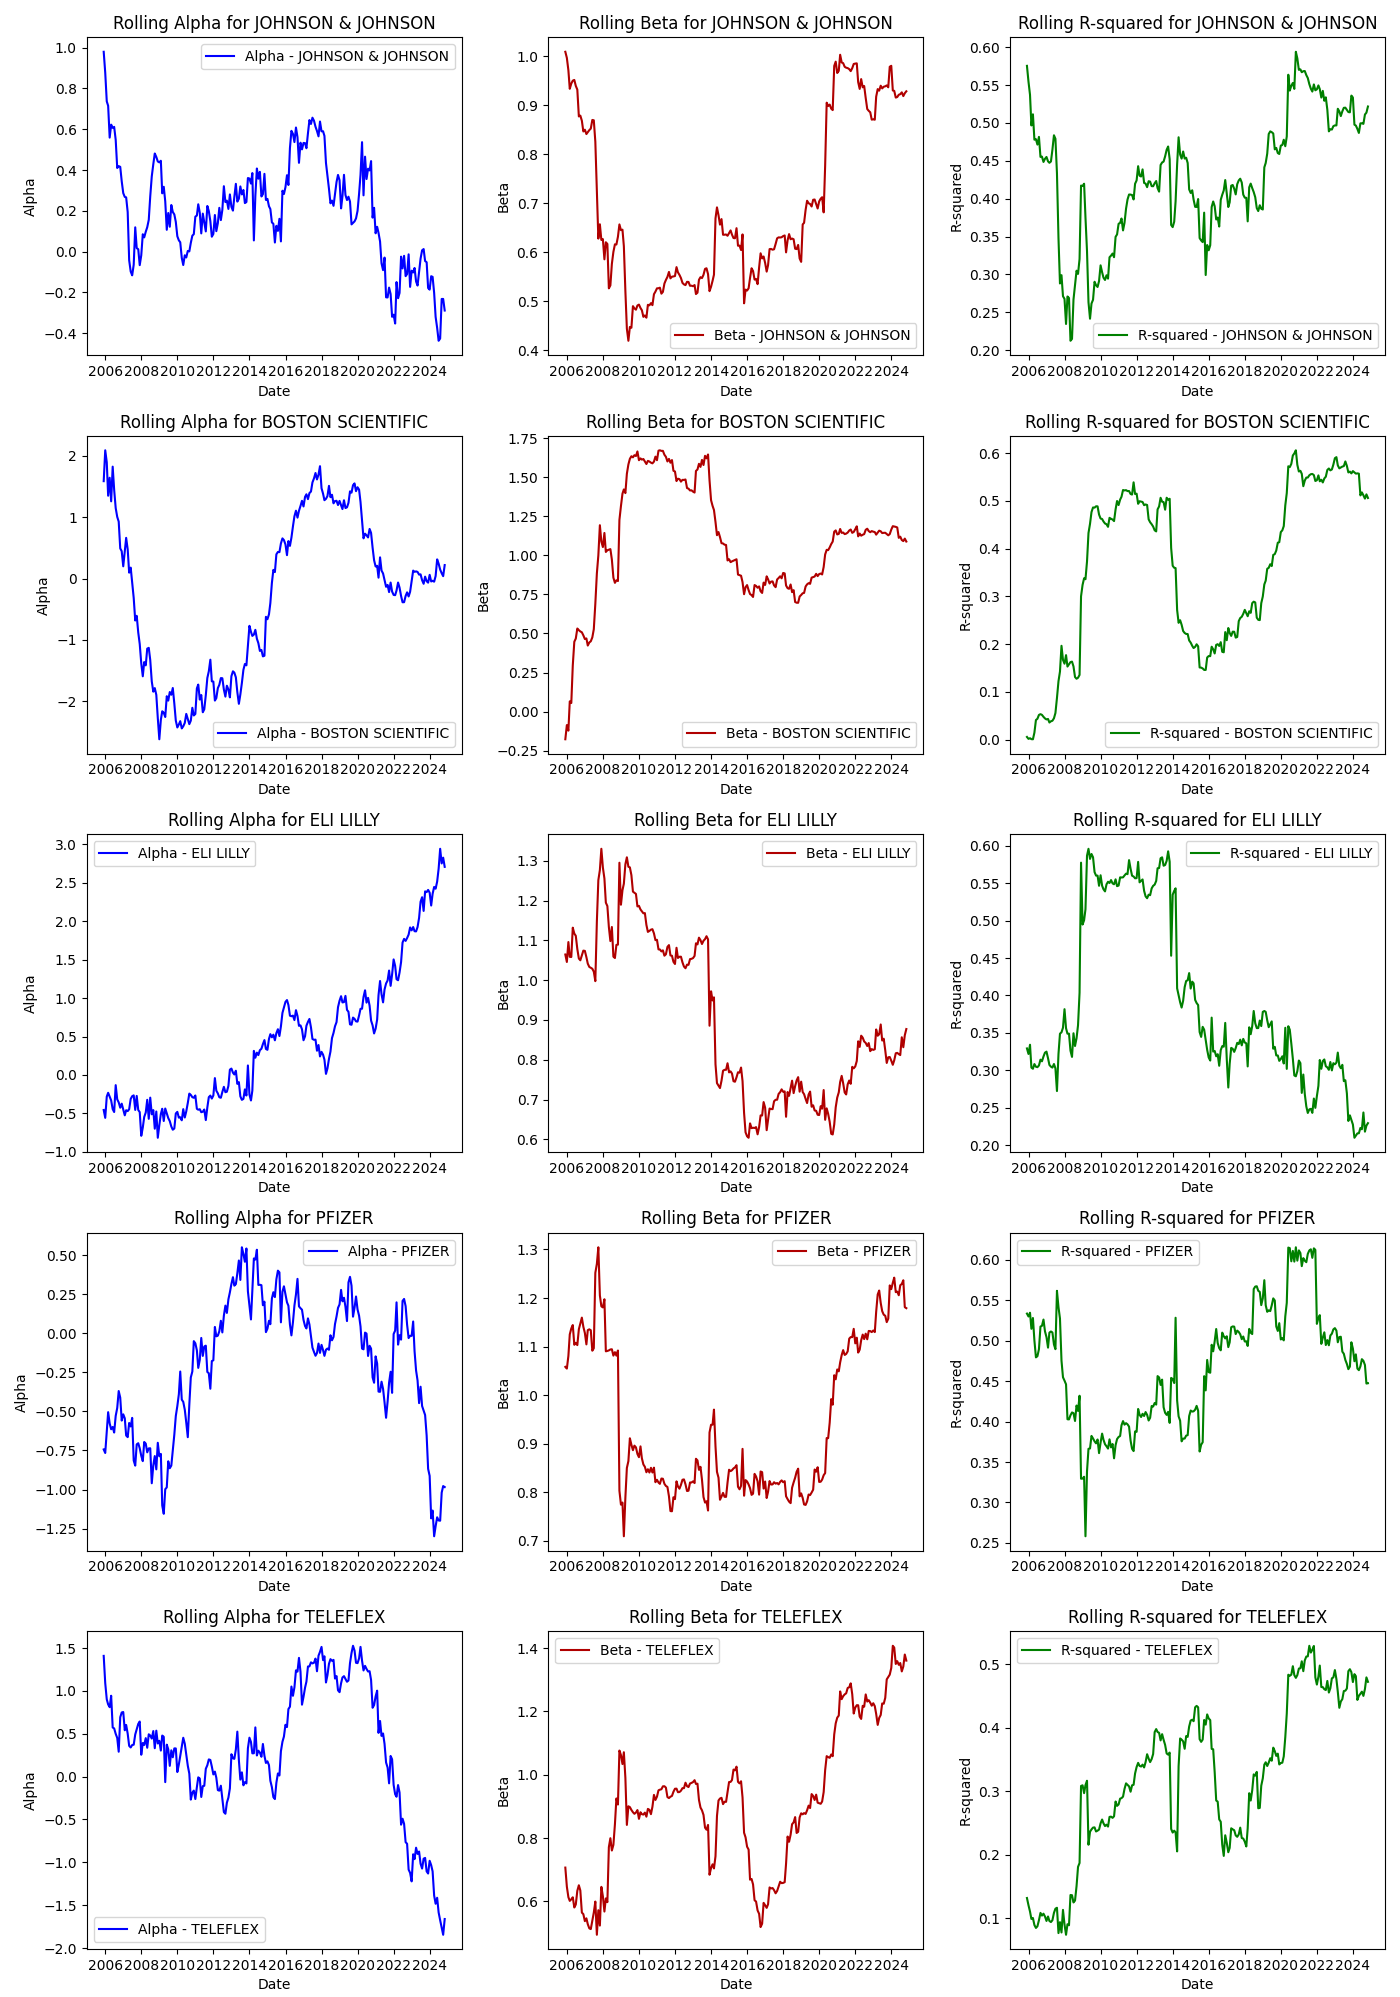
\includegraphics[width=0.8\textwidth]{images/rolling_quantities_1.png}
    \caption{Rolling quantities computed an all equities as an alternative of the Chow Test in search for structural
    breaks (1).}\label{fig:rolling_quantities_1}
\end{figure}
\begin{figure}[h]
    \centering
    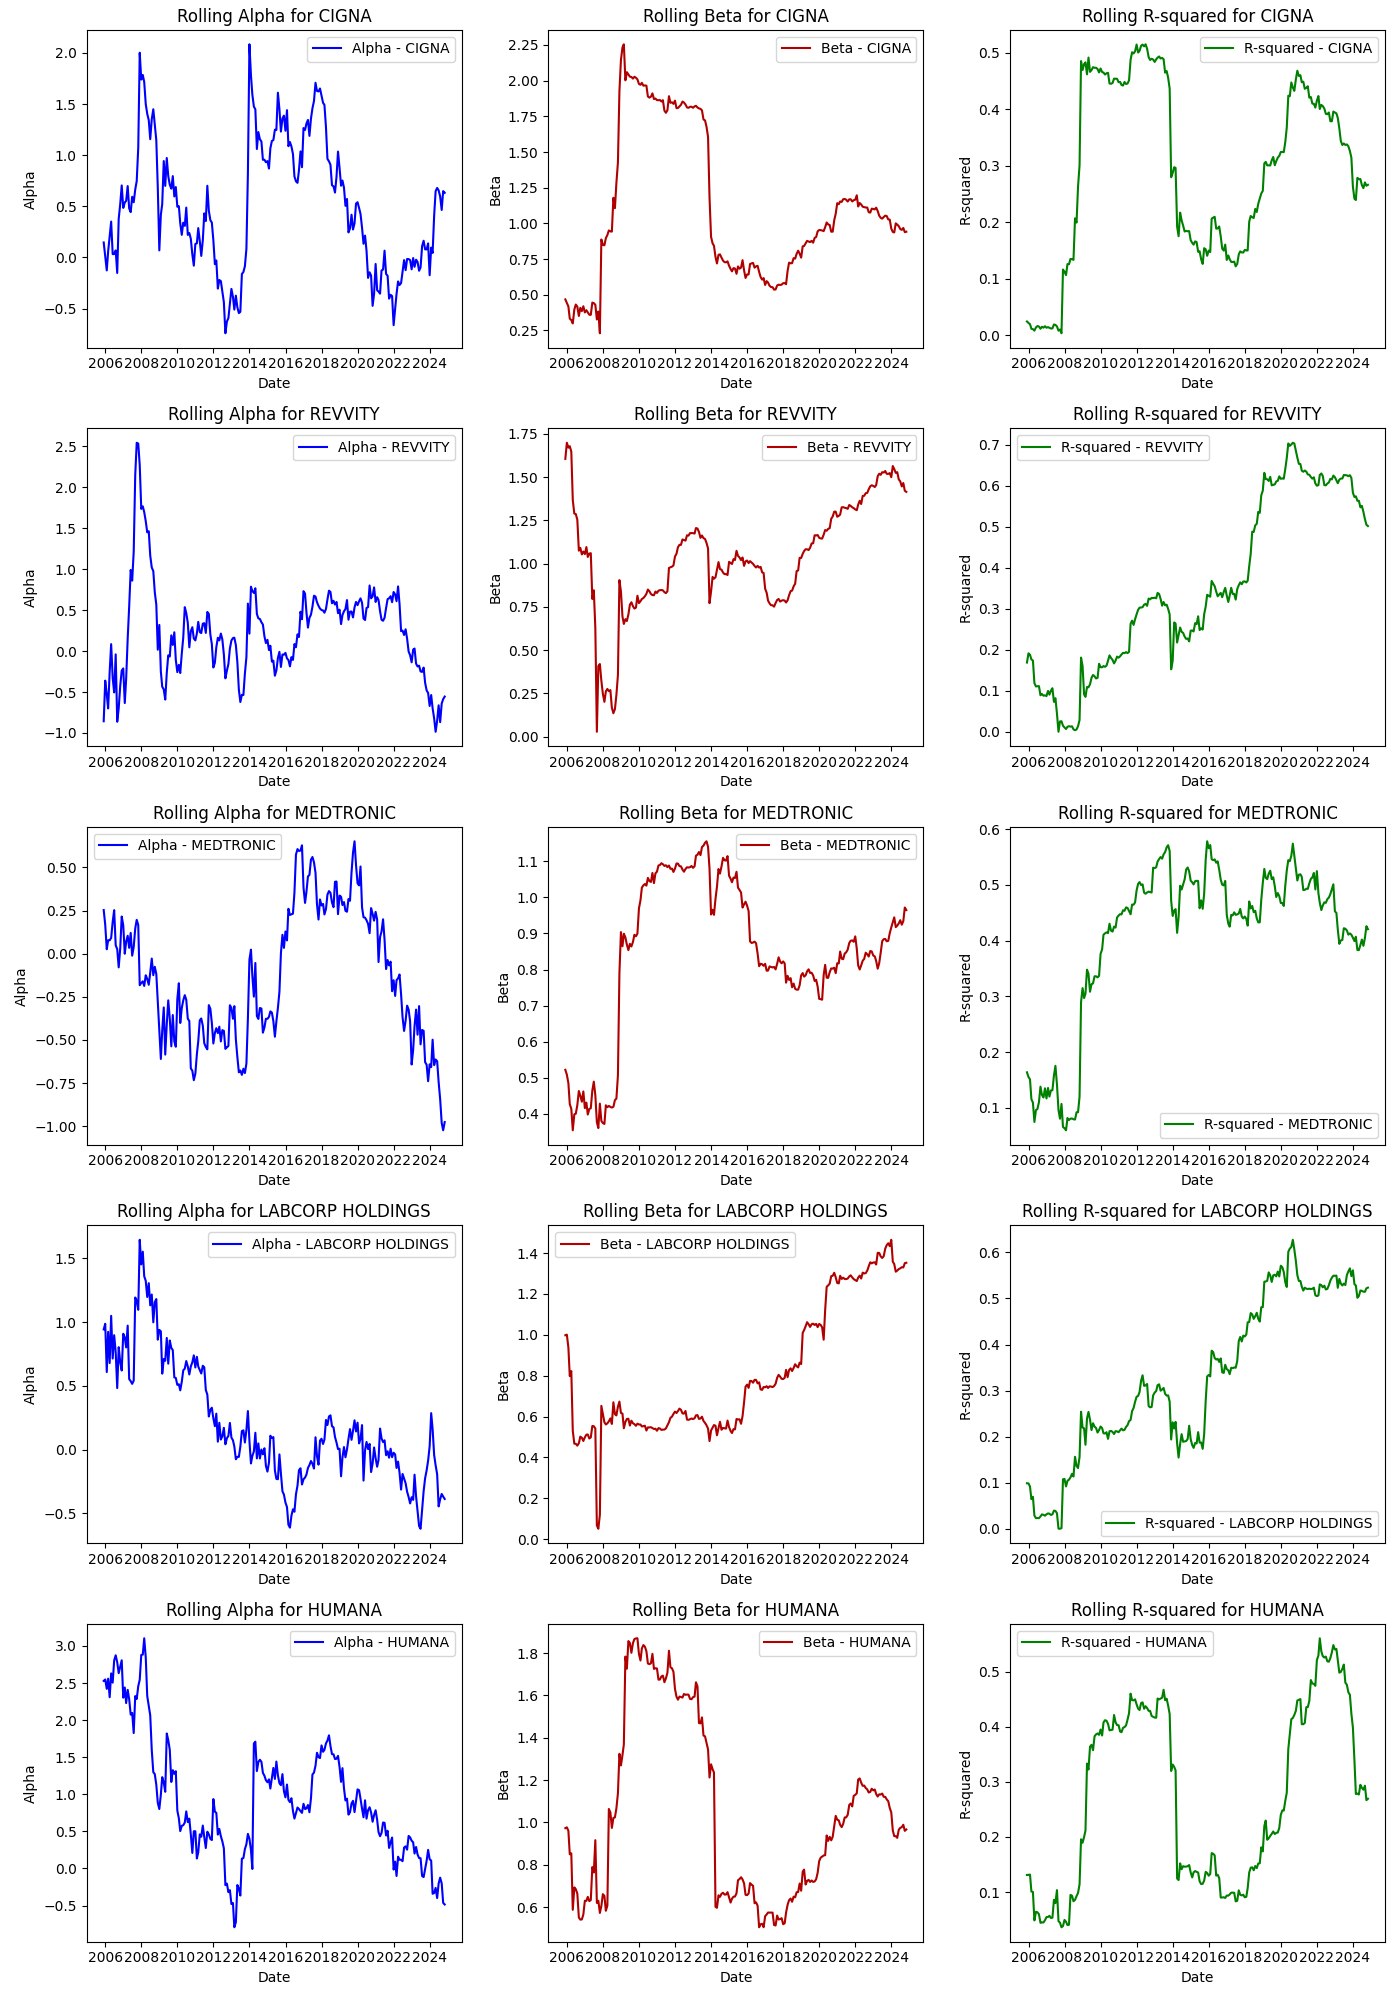
\includegraphics[width=0.8\textwidth]{images/rolling_quantities_2.png}
    \caption{Rolling quantities computed an all equities as an alternative of the Chow Test in search for structural
    breaks (2).}\label{fig:rolling_quantities_2}
\end{figure}

%-------- Assignment 7 -----------------------------------------------------------------------------------------------------%
\section*{Assignment 7}

\begin{figure}[h]
    \centering
    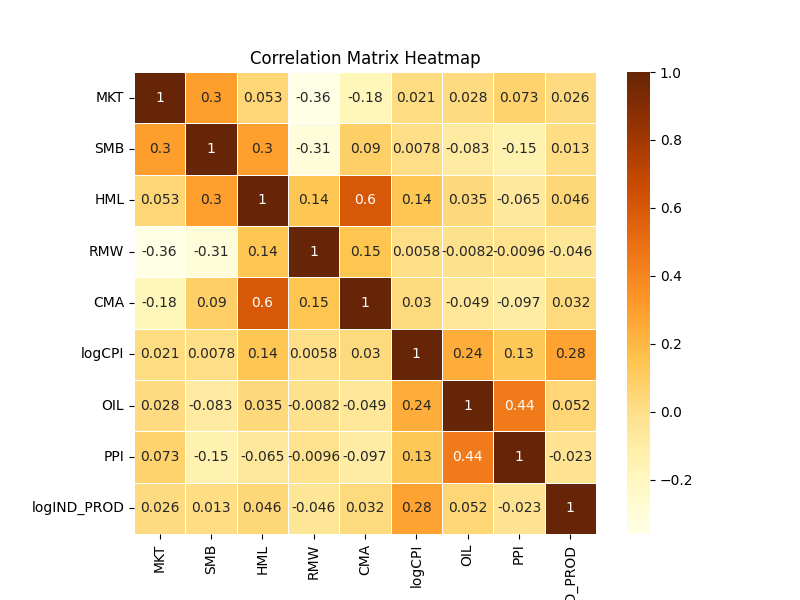
\includegraphics[width=0.8\textwidth]{images/Correlation_heatmap.png}
    \caption{Heatmap of the correlations between the chosen explainatory variables.}\label{fig:Correlation_heatmap}
\end{figure}
%-------- Appendix --------------------------------------------------------------------------------------------------------%
\section*{Appendix}

%-------- Roles Summary ---------------------------------------------------------------------------------------------------%
\section*{Summary of Group Members' Contribution}

\textbf{Martina Arrighini:}\\
\textbf{Luigi Babiski Arruda:}\\ 
\textbf{Giorgio Cottini:}\\
\textbf{Enrico Paciaroni:}\\

%---------------------------------------------------------------------------------------------------------------------------%

\end{document}